\documentclass[11pt]{article}
\usepackage[margin=1in]{geometry}
\usepackage{amsmath,amssymb,amsthm,mathtools}
\usepackage{booktabs}
\usepackage{graphicx}
\usepackage{tikz}
\usetikzlibrary{arrows.meta,positioning,backgrounds}
\usepackage{hyperref}
\usepackage{longtable}
\usepackage{array}
\newtheorem{theorem}{Theorem}
\newtheorem{lemma}[theorem]{Lemma}
\newtheorem{proposition}[theorem]{Proposition}
\newtheorem{corollary}[theorem]{Corollary}
\newtheorem{definition}[theorem]{Definition}
\newtheorem{remark}[theorem]{Remark}
\newenvironment{sourceresult}[1]{\par\medskip\noindent\textbf{#1.}\ \itshape}{\par\medskip}
\sloppy
\emergencystretch=3em

\title{Formal Verification Report: powers\_of\_two\_reach\_one}
\author{Black Swan Labs FCVE \\ ledger through EVENT-016}
\date{2026-09-19}
\begin{document}
\maketitle

\noindent\textbf{Trust Statement.} The formal result was checked using Lean 4.34.0 under the pinned project environment (Mathlib master 5ed2965). The theorem CLAIM-002 was kernel-checked with axiom footprint propext, Quot.sound. Independent checking status is INDEPENDENTLY\_CHECKED (recorded before the Section 17 vocabulary existed, as PASS). Computational/adversarial testing produced: COMPUTATIONALLY\_SUPPORTED; NO\_COUNTEREXAMPLE\_FOUND\_IN\_TESTED\_DOMAIN (diagnostic only). The remaining trust limitations are: The repository, commit and project location were not recorded for this run, so the build cannot be reproduced exactly from this report; The checker used for the independent check is not identified in the record; only its result is. This report does not claim that computational testing constitutes formal proof or that formalization alone establishes the truth of the original informal statement.

\begin{abstract}
This report documents the formal verification of powers\_of\_two\_reach\_one (CLAIM-002) under the Formal Claim Verification Engine. Recorded: build PASS -- 8924/8924 jobs, exit 0, no sorry/admit; axiom footprint propext, Quot.sound; independent check PASS. Computational testing is diagnostic and is not proof. Section 17 states the status the recorded evidence permits; the governance decision is recorded separately, after this report.
\end{abstract}

\section{Mathematical Statement}
\begin{sourceresult}{powers\_of\_two\_reach\_one}
Every power of two reaches 1 under the standard Collatz function: for f(n) = n/2 if n even, 3n+1 if n odd, and for every k >= 0, iterating f starting from 2\textasciicircum{}k eventually reaches 1.
\end{sourceresult}
Source location: source/original.md.

\section{Definitions and Assumptions}
\subsection*{Definitions}
\begin{itemize}
\item f: N -> N (called collatzStep in the Lean formalization), f(n) = n/2 if n even, 3n+1 if n odd -- this is the STANDARD (uncompressed) Collatz map, distinct from Eliahou's compressed map T used in VCE-001
\end{itemize}
\subsection*{Source assumptions}
\begin{itemize}
\item \textbf{SA-001} k is a natural number, k >= 0
\end{itemize}
\subsection*{Formalization assumptions}
\begin{itemize}
\item \textbf{FA-001} 'iterating f m times' is represented via Mathlib's Function.iterate (f\textasciicircum{}[m]), a standard, well-understood construction with no hidden semantics beyond repeated function application
\end{itemize}
\subsection*{Computational assumptions}
None recorded.
\section{Proof Outline}
\begin{enumerate}
\item \textbf{method.} induction on k
\item \textbf{base case.} k=0: 2\textasciicircum{}0=1, already at 1 in 0 steps
\item \textbf{inductive step.} 2\textasciicircum{}(k+1) is even, one step of f sends it to 2\textasciicircum{}k; by induction hypothesis 2\textasciicircum{}k reaches 1 in m more steps, so 2\textasciicircum{}(k+1) reaches 1 in m+1 steps
\end{enumerate}
\section{Proof Dependency Diagram}
\begin{center}
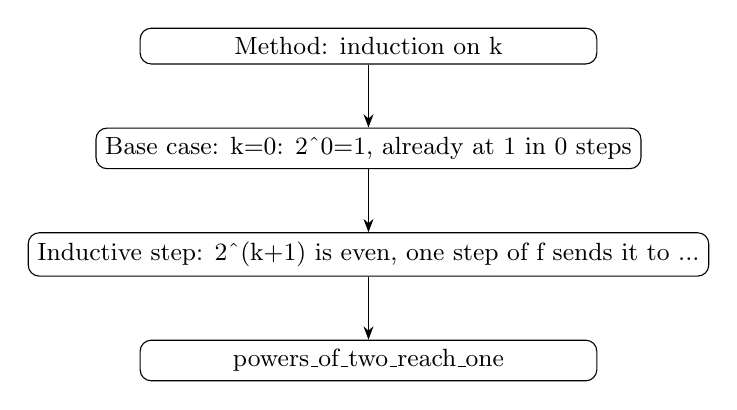
\begin{tikzpicture}[box/.style={draw,rounded corners,align=center,minimum width=58mm,font=\small}, node distance=8mm, >=Stealth]
\node[box] (s0) {Method: induction on k};
\node[box, below=of s0] (s1) {Base case: k=0: 2\textasciicircum{}0=1, already at 1 in 0 steps};
\draw[->] (s0) -- (s1);
\node[box, below=of s1] (s2) {Inductive step: 2\textasciicircum{}(k+1) is even, one step of f sends it to ...};
\draw[->] (s1) -- (s2);
\node[box, below=of s2] (goal) {powers\_of\_two\_reach\_one};
\draw[->] (s2) -- (goal);
\end{tikzpicture}
\end{center}
\section{Formalization}
Lean identifiers below are cross-references; the mathematics is in the sections above (\S{}29).
\subsection*{powers\_of\_two\_reach\_one}
{\footnotesize\ttfamily\raggedright\hangindent=1.4em\hangafter=1\noindent
\hspace*{0.00em}theorem powers\_\allowbreak{}of\_\allowbreak{}two\_\allowbreak{}reach\_\allowbreak{}one : \ensuremath{\forall} k : \ensuremath{\mathbb{N}}, \ensuremath{\exists} m : \ensuremath{\mathbb{N}}, (collatzStep\textasciicircum{}[m]) (2 \textasciicircum{} k) = 1\par
}

\section{Semantic Bridge}
\subsection*{Informal Statement}
Every power of two reaches 1 under the standard Collatz function: for f(n) = n/2 if n even, 3n+1 if n odd, and for every k >= 0, iterating f starting from 2\textasciicircum{}k eventually reaches 1.
\subsection*{Normalized Statement}
\subsection*{Normalized Claim: CLAIM-002}
\subsubsection*{Objects and domains}
\begin{itemize}
\item $f : \mathbb{N} \to \mathbb{N}$, $f(n) = \begin{cases} n/2 & n \text{ even} \\ 3n+1 & n \text{ odd} \end{cases}$ --- the \textbf{standard} (uncompressed) Collatz map. (Note: this is a different map from Eliahou's compressed $T$ used in VCE-001, which folds the forced halving after an odd step into one combined step. $f$ and $T$ are related but not identical.)
\item $f^{(m)}$ denotes $f$ composed with itself $m$ times.
\end{itemize}
\subsubsection*{The claim}
\textbf{Given}: $k \in \mathbb{N}$.

\textbf{Conclusion}: $\exists\, m \in \mathbb{N}$ such that $f^{(m)}(2^k) = 1$.

\subsubsection*{Why this is true}
By induction on $k$.

\begin{itemize}
\item \textbf{Base case} ($k=0$): $2^0 = 1$, so $m=0$ works trivially.
\item \textbf{Inductive step}: assume $f^{(m)}(2^k) = 1$ for some $m$. Since $2^{k+1}$ is even, $f(2^{k+1}) = 2^{k+1}/2 = 2^k$. So $f^{(m+1)}(2^{k+1}) = f^{(m)}(f(2^{k+1})) = f^{(m)}(2^k) = 1$.
\end{itemize}
This is a completely elementary, fully constructive argument --- no case analysis beyond parity, no external results needed.

\subsubsection*{Status}
\textbf{MATCH} --- direct restatement, nothing to disambiguate.


\subsection*{Lean Statement}
{\footnotesize\ttfamily\raggedright\hangindent=1.4em\hangafter=1\noindent
\hspace*{0.00em}theorem powers\_\allowbreak{}of\_\allowbreak{}two\_\allowbreak{}reach\_\allowbreak{}one : \ensuremath{\forall} k : \ensuremath{\mathbb{N}}, \ensuremath{\exists} m : \ensuremath{\mathbb{N}}, (collatzStep\textasciicircum{}[m]) (2 \textasciicircum{} k) = 1\par
}

\subsection*{Differences}
\subsection*{Gate 4: Lean Formalization Comparison --- CLAIM-002}
\begin{center}\small\begin{tabular}{p{0.46\textwidth}p{0.46\textwidth}}\toprule
Human mathematics (normalized) & Lean \\ \midrule
$f(n) = n/2$ if even, $3n+1$ if odd & \texttt{def collatzStep (n : \ensuremath{\mathbb{N}}) : \ensuremath{\mathbb{N}} := if n \% 2 = 0 then n / 2 else 3 * n + 1} \\
$\forall k,\ \exists m,\ f^{(m)}(2^k)=1$ & \texttt{theorem powers\_of\_two\_reach\_one : \ensuremath{\forall} k : \ensuremath{\mathbb{N}}, \ensuremath{\exists} m : \ensuremath{\mathbb{N}}, (collatzStep\textasciicircum{}[m]) (2 \textasciicircum{} k) = 1} \\
Induction on $k$, base case $2^0=1$, step: $2^{k+1}\to 2^k$ via one even step & \texttt{induction k with | zero => exact \ensuremath{\langle}0, rfl\ensuremath{\rangle} | succ n ih => ...} --- identical structure \\
\bottomrule\end{tabular}\end{center}
\subsubsection*{Checklist}
\begin{center}\small\begin{tabular}{p{0.46\textwidth}p{0.46\textwidth}}\toprule
Check & Finding \\ \midrule
Stronger/weaker & Neither --- exact match \\
Altered domain & No \\
Missing/extra hypothesis & None \\
Changed quantifier & No \\
Changed function & No --- \texttt{collatzStep} is exactly $f$ as normalized \\
Coercion & None needed (pure \ensuremath{\mathbb{N}} arithmetic throughout) \\
Finite/infinite mismatch & No \\
\bottomrule\end{tabular}\end{center}
This is the simplest possible Gate 4 outcome: the Lean statement is a direct

transliteration of the normalized claim, and the proof's induction structure

matches the normalized proof step-for-step (base case \texttt{k=0}, inductive step

using \texttt{Function.iterate\_succ} to peel off exactly one application of

\texttt{collatzStep}, matching the normalized argument's "$f(2^{k+1})=2^k$, then

apply the inductive hypothesis").

\subsubsection*{Status: MATCH}

\subsection*{Findings recorded by the reviewer}
No difference was found by any of the required checks; each check records its basis in the semantic record.
\subsection*{Justification}
Gate 4 records the Lean statement as a direct transliteration of the normalized claim (same function, domain, quantifiers, conclusion) and the proof's induction structure matches the normalized argument step for step. The Gate 7 re-audit found no undisclosed change, and the axiom footprint contains no classical assumption.


\subsection*{Verdict}
\noindent\textbf{FAITHFUL}\par Set by Wilson. Recorded context: Gate 4 recorded MATCH; Gate 7 recorded PASS -- no undisclosed semantic change; axiom footprint itself serves as independent corroboration of the re-audit's conclusion.
\section{Lean Environment}
\begin{tabular}{@{}ll@{}}
\toprule
Lean Version & 4.34.0 \\
Mathlib Version & master 5ed2965 \\
\bottomrule
\end{tabular}
\section{Formal Verification}
PASS -- 8924/8924 jobs, exit 0, no sorry/admit.
Source of this field: ledger:EVENT-006.
\section{Axiom Audit}
Actual axiom footprint: propext, Quot.sound.
Source: parsed-legacy-text:EVENT-007.
\section{Independent Check}
PASS -- Checked 1662 declarations with no errors. Axioms confirmed: propext, Quot.sound (matches Gate 6 exactly).  (legacy wording).
Recording the checker and its version does not by itself establish independence (\S{}17).
\section{Computational / Adversarial Tests}
Counterexample search: COMPUTATIONALLY\_SUPPORTED -- all cases reach 1 in exactly k steps as predicted; no counterexample in tested domain [diagnostic, not proof]

Computational test: NO\_COUNTEREXAMPLE\_FOUND\_IN\_TESTED\_DOMAIN -- 5001 cases over: every integer k in [0,5000]; full trajectory 2\textasciicircum{}k..1; two independent implementations of f; NOT PROOF [diagnostic, not proof]

Neither result is formal proof (\S{}16, \S{}18).

Tested domain: every integer k in [0,5000]; full trajectory 2\textasciicircum{}k..1; two independent implementations of f; cases: 5001; categories not covered: degenerate, empty, singleton, domain\_transition, pathological.
\section{Verification Limitations}
\begin{longtable}{p{0.16\textwidth}p{0.78\textwidth}}
\toprule Item & Limitation \\ \midrule \endhead
1 & The repository, commit and project location were not recorded for this run, so the build cannot be reproduced exactly from this report. \\
2 & The checker used for the independent check is not identified in the record; only its result is. \\
\midrule \multicolumn{2}{l}{\textit{Record-keeping notes (these do not change what the verification shows)}} \\ \midrule
3 & 10 of 16 ledger events predate the input/output hash fields and carry none. \\
4 & Events EVENT-009 (COMPUTATIONALLY\_SUPPORTED) used wording outside the Section 16 vocabulary; each is read as diagnostic evidence, not proof. \\
\bottomrule
\end{longtable}
\section{Verification Matrix}
\begin{longtable}{lllll}
\toprule Gate & Ledger action & Event & Status & Satisfied \\ \midrule \endhead
G0 & source intake & EVENT-001 & PASS & yes \\
G1 & claim extraction & EVENT-002 & PASS & yes \\
G2 & assumption extraction & EVENT-003 & PASS & yes \\
G3 & semantic normalization & EVENT-004 & PASS & yes \\
G4 & lean formalization comparison & EVENT-005 & PASS & yes \\
G5 & lean build & EVENT-006 & PASS & yes \\
G6 & axiom audit & EVENT-007 & PASS & yes \\
G7 & semantic re audit & EVENT-008 & PASS & yes \\
G8 & adversarial computational test & EVENT-009 & DIAGNOSTIC & yes \\
G9 & independent check & EVENT-010 & PASS & yes \\
G10 & computational check & EVENT-011 & DIAGNOSTIC & yes \\
G11 & evidence graph & EVENT-012 & PASS & yes \\
G12 & report generation & EVENT-014 & PASS & yes \\
ORDER & canonical chain (\S{}2) & - & PASS & yes \\
\bottomrule
\end{longtable}
\section{Trust / Verification Chain}
\begin{center}
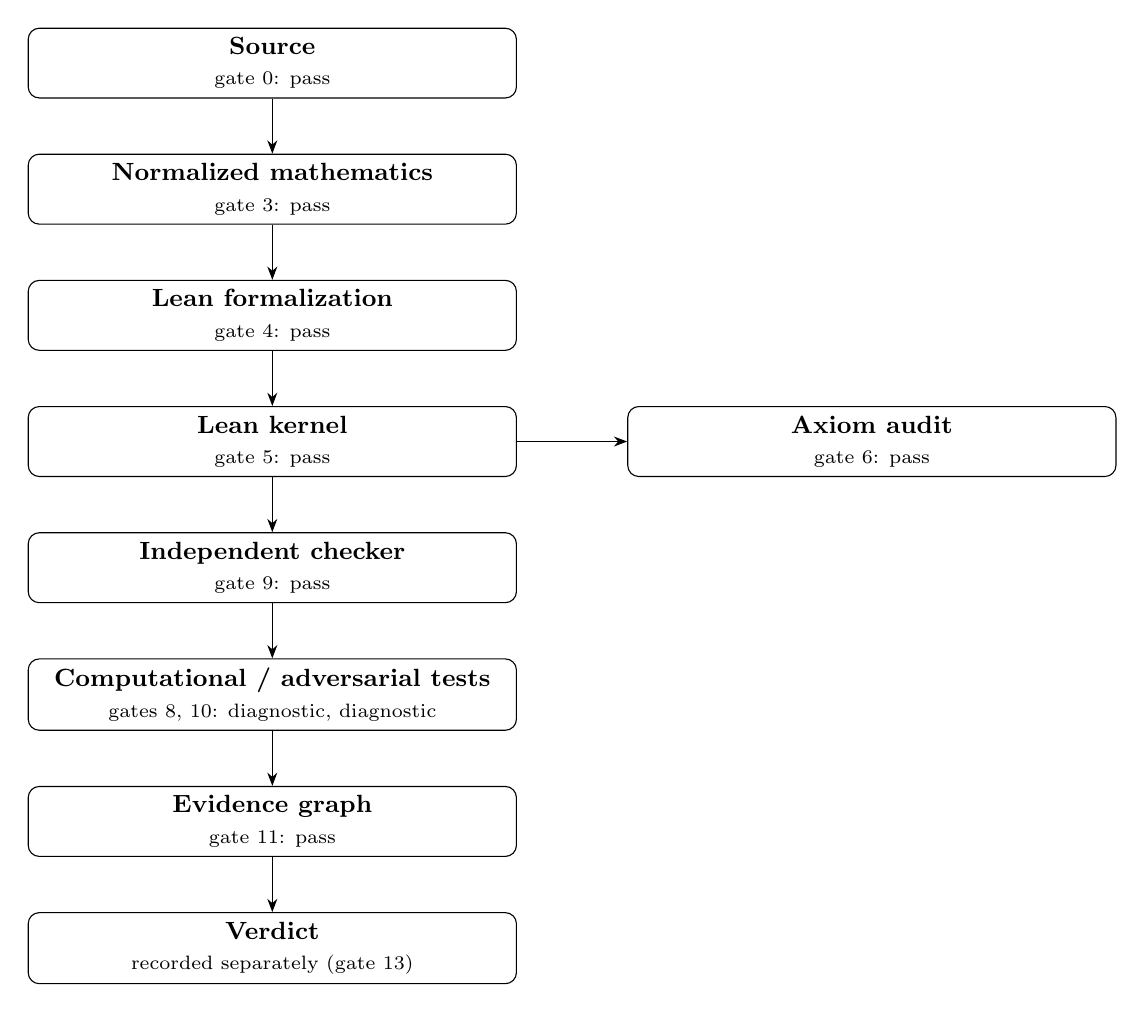
\begin{tikzpicture}[node distance=7mm, box/.style={draw,rounded corners,align=center,minimum width=62mm,font=\small}, >=Stealth]
\node[box] (src) {\textbf{Source}\\{\scriptsize gate 0: pass}};
\node[box, below=of src] (norm) {\textbf{Normalized mathematics}\\{\scriptsize gate 3: pass}};
\draw[->] (src) -- (norm);
\node[box, below=of norm] (lean) {\textbf{Lean formalization}\\{\scriptsize gate 4: pass}};
\draw[->] (norm) -- (lean);
\node[box, below=of lean] (kern) {\textbf{Lean kernel}\\{\scriptsize gate 5: pass}};
\draw[->] (lean) -- (kern);
\node[box, below=of kern] (chk) {\textbf{Independent checker}\\{\scriptsize gate 9: pass}};
\draw[->] (kern) -- (chk);
\node[box, below=of chk] (comp) {\textbf{Computational / adversarial tests}\\{\scriptsize gates 8, 10: diagnostic, diagnostic}};
\draw[->] (chk) -- (comp);
\node[box, below=of comp] (evd) {\textbf{Evidence graph}\\{\scriptsize gate 11: pass}};
\draw[->] (comp) -- (evd);
\node[box, below=of evd] (ver) {\textbf{Verdict}\\{\scriptsize recorded separately (gate 13)}};
\draw[->] (evd) -- (ver);
\node[box, right=14mm of kern] (ax) {\textbf{Axiom audit}\\{\scriptsize gate 6: pass}};
\draw[->] (kern) -- (ax);
\end{tikzpicture}
\end{center}
\section{Reproducibility Instructions}
\begin{tabular}{@{}p{0.27\textwidth}p{0.68\textwidth}@{}}
\toprule
Repository URL & NOT RECORDED \\
Commit & NOT RECORDED \\
Project directory when run & NOT RECORDED \\
Lean toolchain file & NOT RECORDED \\
Lean version & 4.34.0 \\
Lake version & NOT RECORDED \\
Mathlib revision & master 5ed2965 \\
Checker & NOT RECORDED \\
Expected build result & PASS -- 8924/8924 jobs, exit 0, no sorry/admit \\
\bottomrule
\end{tabular}

{\footnotesize\ttfamily\raggedright\hangindent=1.4em\hangafter=1\noindent
\hspace*{0.00em}\# repository location and commit were not recorded for this run (see table above)\par
\hspace*{0.00em}cat lean-toolchain\par
\hspace*{0.00em}lake --version\par
\hspace*{0.00em}lean --version\par
\hspace*{0.00em}lake build\par
\hspace*{0.00em}\# in a Lean file importing the module:  \#print axioms powers\_\allowbreak{}of\_\allowbreak{}two\_\allowbreak{}reach\_\allowbreak{}one\par
\hspace*{0.00em}\# independent-check commands were not recorded for this run\par
}

This run predates structured build records, so the repository, commit and project location above are NOT RECORDED; the commands are the generic sequence, not an exact recipe.
Reproducibility level supported by recorded evidence: R4. This tool did not re-run the build.
\section{Correction Ledger}
No failed or unresolved gate results are recorded in the ledger.
\subsection*{Correction Ledger --- VCE-002 rev r}
\subsubsection*{CORRECTION-001 --- first attempt superseded}
\begin{itemize}
\item \textbf{original\_claim}: the first build of this run (archived at \texttt{verification-002r-attempt1-superseded/}) produced a report saying ``Promotion is not supported because: G12 (report generation): missing''.
\item \textbf{error}: false. Every gate except the governance decision (G13) was satisfied.
\item \textbf{detection\_method}: reading the rendered PDF after verifying the ledger and gate table; the report's claim disagreed with the \S{}53 table.
\item \textbf{root\_cause}: \texttt{permitted\_status} counted G12 as a blocker, but a report is built before its own Gate 12 event exists, so G12 was always ``missing'' at that moment (a circularity in the tool).
\item \textbf{repair}: G12 is ignored when the report computes what the evidence permits; the report states the assumption that it compiles cleanly. Same-day regression tests added.
\item \textbf{recheck}: the whole run was rebuilt from the same first ten events (hashes identical) and re-verified: chain intact, canonical order, graph current.
\item \textbf{result}: RESOLVED. The first attempt is kept, not deleted.
\item \textbf{date}: 2026-09-19
\end{itemize}
\subsubsection*{CORRECTION-002 --- report EVENT-013 superseded by EVENT-014}
\begin{itemize}
\item \textbf{original\_claim}: report EVENT-013 was correct.
\item \textbf{error}: it printed a literal ``\textbackslash{}S 53'' in the permitted-status paragraph (a doubly escaped section sign). Cosmetic; no fact was wrong.
\item \textbf{detection\_method}: reading the rendered PDF text.
\item \textbf{root\_cause}: a \texttt{\textbackslash{}S} written into text that is then LaTeX-escaped.
\item \textbf{repair}: the wording now reads ``Section 53''; Gate 12 was re-run, appending EVENT-014. EVENT-013 stays in the ledger; EVENT-014 supersedes it.
\item \textbf{recheck}: the regenerated PDF was read again.
\item \textbf{result}: RESOLVED.
\item \textbf{date}: 2026-09-19
\end{itemize}
\subsubsection*{CORRECTION-003 --- decision EVENT-015 superseded by EVENT-016 (mistyped input ids)}
\begin{itemize}
\item \textbf{original\_claim}: decision EVENT-015 (PROMOTE, recorded on Wilson's instruction) was a valid record.
\item \textbf{error}: its inputs were \texttt{GRAPH-002,REPORT-002}, but this run's nodes are \texttt{GRAPH-002r} and \texttt{REPORT-002r}. The ids named nothing, so the v3 graph had dangling edges, G11 failed, and the receipt generated from it reported ``PROMOTE not supported by \S{}53: G11'' --- a true statement about a malformed record, not about the evidence. The decision itself (PROMOTE, by Wilson) was unaffected.
\item \textbf{detection\_method}: the receipt's own decision check (\texttt{fcve\_receipt.check\_decision}) on first generation.
\item \textbf{root\_cause}: (1) the assistant typed the wrong input ids; (2) nothing checked input ids at append time; (3) the graph builder kept the edges of superseded events, so a superseding event could not have cleared the dangling edges.
\item \textbf{repair}: EVENT-016 re-records the same decision with the correct inputs; EVENT-015 stays in the ledger. The graph now drops superseded events; \texttt{append} now refuses an input id no earlier event produced (\texttt{check\_inputs}, on in the CLI and batch). The flawed receipt is archived in \texttt{receipt/superseded-EVENT-015/}, not deleted, and the receipt regenerated.
\item \textbf{recheck}: chain, order, graph and receipt re-verified after the correction.
\item \textbf{result}: RESOLVED.
\item \textbf{date}: 2026-09-19
\end{itemize}


\section{Conclusion}
The recorded evidence is summarized in the Trust Statement and the verification matrix above. Recorded failure is not a passed gate.
\begin{center}\begin{tabular}{@{}p{0.36\textwidth}p{0.58\textwidth}@{}}
FORMAL PROOF (build): & PASS \\
AXIOM AUDIT: & PASS \\
SEMANTIC MATCH (Gate 4): & PASS \\
SEMANTIC RE-AUDIT (Gate 7): & PASS \\
INDEPENDENT CHECK: & PASS \\
COUNTEREXAMPLE SEARCH: & NO COUNTEREXAMPLE FOUND IN TESTED DOMAIN (diagnostic, not proof) \\
COMPUTATIONAL TEST: & NO COUNTEREXAMPLE FOUND IN TESTED DOMAIN (diagnostic, not proof) \\
REPRODUCIBILITY: & R4 (ceiling supported by recorded evidence) \\
\end{tabular}\end{center}
%% PERMITTED-STATUS-BEGIN
\begin{quote}\textbf{Status the evidence permits.} The recorded evidence satisfies the conditions for promotion (Section 53). Whether to promote is the reviewer's decision, recorded after this report. This is not a decision: the governance decision is recorded as a separate step after this report.\end{quote}
%% PERMITTED-STATUS-END
\appendix
\section{Lean Source}
{\footnotesize\ttfamily\raggedright\hangindent=1.4em\hangafter=1\noindent
\hspace*{0.00em}theorem powers\_\allowbreak{}of\_\allowbreak{}two\_\allowbreak{}reach\_\allowbreak{}one : \ensuremath{\forall} k : \ensuremath{\mathbb{N}}, \ensuremath{\exists} m : \ensuremath{\mathbb{N}}, (collatzStep\textasciicircum{}[m]) (2 \textasciicircum{} k) = 1\par
}

\section{Tests}
\begin{itemize}
\item \textbf{EVENT-009} python3 verification-002/computational/tests/verify\_powers\_of\_two.py: COMPUTATIONALLY\_SUPPORTED -- all cases reach 1 in exactly k steps as predicted; no counterexample in tested domain
\item \textbf{EVENT-011} python Python 3.12.9: verify\_gate10.py: NO\_COUNTEREXAMPLE\_FOUND\_IN\_TESTED\_DOMAIN -- 5001 cases over: every integer k in [0,5000]; full trajectory 2\textasciicircum{}k..1; two independent implementations of f; NOT PROOF
\end{itemize}
\section{Evidence Receipt}
\begin{longtable}{p{0.24\textwidth}p{0.70\textwidth}}
\toprule Field & Value \\ \midrule \endhead
SOURCE HASH & sha256:97d49fb\allowbreak{}c3576e79f3901c\allowbreak{}e85f0fb9dd92d9\allowbreak{}cbf06d6beb933a\allowbreak{}ada6a2f1a194d6\allowbreak{}0 (../verificati\allowbreak{}on-002/source/\allowbreak{}original.md) \\
THEOREM ID & CLAIM-002 (powers\_of\_two\allowbreak{}\_reach\_one) \\
CLAIM & Every power of two reaches 1 under the standard Collatz function: for f(n) = n/2 if n even, 3n+1 if n odd, and for every k >= 0, iterating f starting from 2\textasciicircum{}k eventually reaches 1. \\
NORMALIZED CLAIM & verification-0\allowbreak{}02/normalized/\allowbreak{}normalized-cla\allowbreak{}im.md -- MATCH \\
LEAN STATEMENT & Gate 4: MATCH \\
LEAN VERSION & 4.34.0 \\
MATHLIB VERSION & master 5ed2965 \\
BUILD RESULT & PASS -- 8924/8924 jobs, exit 0, no sorry/admit \\
AXIOM FOOTPRINT & propext, Quot.sound \\
INDEPENDENT CHECK & PASS -- Checked 1662 declarations with no errors. Axioms confirmed: propext, Quot.sound (matches Gate 6 exactly).  (legacy wording) \\
COMPUTATIONAL TEST & NO\_COUNTEREXAM\allowbreak{}PLE\_FOUND\_IN\_T\allowbreak{}ESTED\_DOMAIN -- 5001 cases over: every integer k in [0,5000]; full trajectory 2\textasciicircum{}k..1; two independent implementation\allowbreak{}s of f; NOT PROOF [diagnostic, not proof] \\
COUNTEREXAMPLE SEARCH & COMPUTATIONALL\allowbreak{}Y\_SUPPORTED -- all cases reach 1 in exactly k steps as predicted; no counterexample in tested domain [diagnostic, not proof] \\
SEMANTIC MATCH & Gate 4: MATCH; Gate 7: PASS -- no undisclosed semantic change; axiom footprint itself serves as independent corroboration of the re-audit's conclusion \\
REPRODUCIBILITY LEVEL & R4 (ceiling supported by recorded evidence; NOT re-run by this tool; R5 needs full-package rebuild, not assessed) \\
GRAPH HASH & v3 97d4d865cec2cd\allowbreak{}c842e0714af1a2\allowbreak{}a030fd62d0397e\allowbreak{}9e7327c9b74ebe\allowbreak{}67a09c54 (covers 16 events through EVENT-016) \\
COST & 16 ledger events; LEAN\_BUILD\_TIM\allowbreak{}E=NOT RECORDED; COMPUTATIONAL\_\allowbreak{}TEST\_TIME=7.19\allowbreak{}; CHECKER\_TIME=N\allowbreak{}OT RECORDED; HUMAN\_TIME, MODEL\_CALL\_COU\allowbreak{}NT, MODEL\_COST, LATEX\_BUILD\_TI\allowbreak{}ME=NOT RECORDED (no cost ledger, \S{}43) \\
\bottomrule
\end{longtable}
\end{document}
